\section{Performance Evaluation}
\label{sec:Performance}

We conducted our tests in two different mode: scan mode, and monitor mode. In scan mode, the relevant portion of the filesystem is scanned and a tree is built of modification times, both locally and on the server.  The server then sends this information down to the local device, where they are compared to determine what needs to be synchronized. In monitor mode, we use filesystem monitors to watch for changed files on both server and client side, so the only files that are considered for synchronization are those which changed. 

%more info is needed here on how the tests were actually carried out

\subsection{Testing Plan}
In our experiments, we ran the Teledroid application on the background. In turn, we updated multiple files, which is a total of 1MB size large, on both local device and server side respectively for three time. In the experiment, we captured the CPU usage and memory usage in every 10 second. After Teledroid completed one round of files transfer, we recorded the time it spent on each round. The experiments were doing in both scan mode and monitor mode.
				
\subsection{Hardware Configuration}
Our test device is an Android Dev Phone 1. It has a 528MHZ Qualcomm 7210 processor and 192 MB RAM. It features a touch screen and a trackball for navigation, and provides QWERTY slider keyboard for input. Wi-Fi, GPS, and Bluetooth v2.0 are also present. It also supports 3G WCDMA in 1700/2100 MHz and Quad-band GSM in 850/900/1800/1900 MHz. Note that the Android Dev Phone 1 includes 1GB MicroSC card as an external storage device. It can be replaced with a card of up to 16GB. Concerning the network environment, our tests utilized the University of San Francisco's internet connection, accessed through 802.11g.

\subsection{Results}
The results of our CPU usage tests are shown in Figure~\ref{fig:cpu}. However it is not as we expected. The monitor mode didn't gain any significant advantage over scan mode. However, synchronization finished faster than in scan mode, so the overall cpu usage should be lower than our tests indicate.

\begin{figure}%[htp]
\centering
\subfigure[CPU Usage in Monitor Mode]{\label{fig:cpu-monitor}
    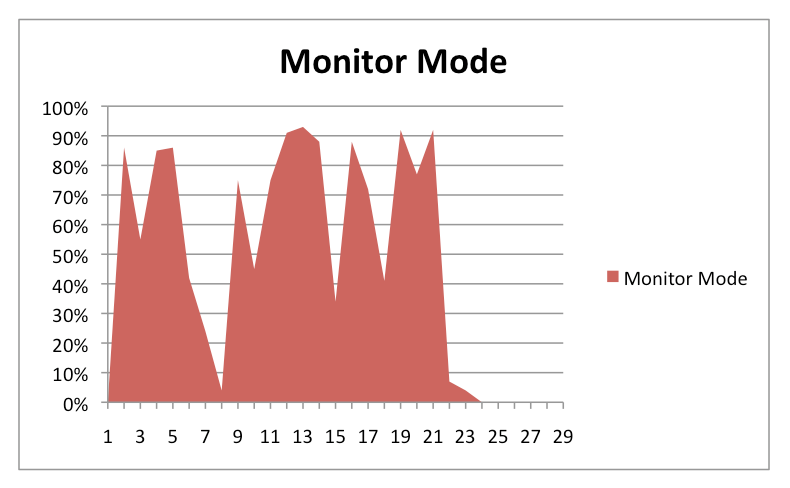
\includegraphics[scale=0.5]{cpu_monitor}}
\hspace{0.20in}
\subfigure[CPU Usage in Scan Mode]{\label{fig:cpu-scan}
	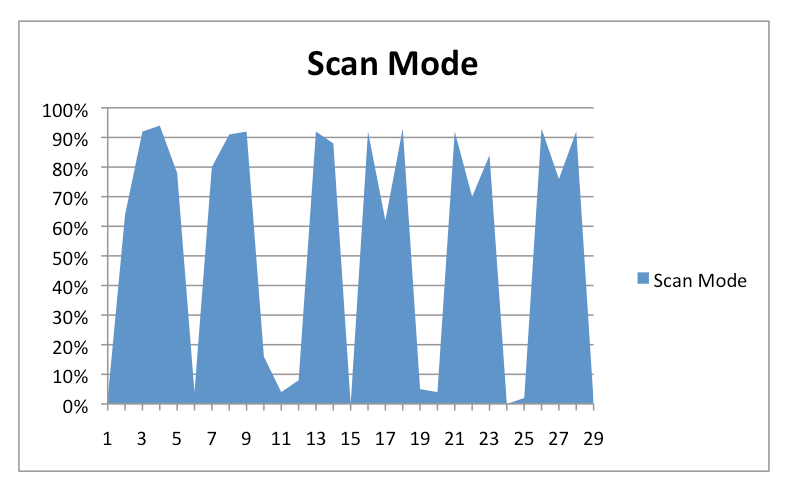
\includegraphics[scale=0.5]{cpu_scan}}
\subfigure[Comparison of CPU Usage]{\label{fig:cpu-comp}
    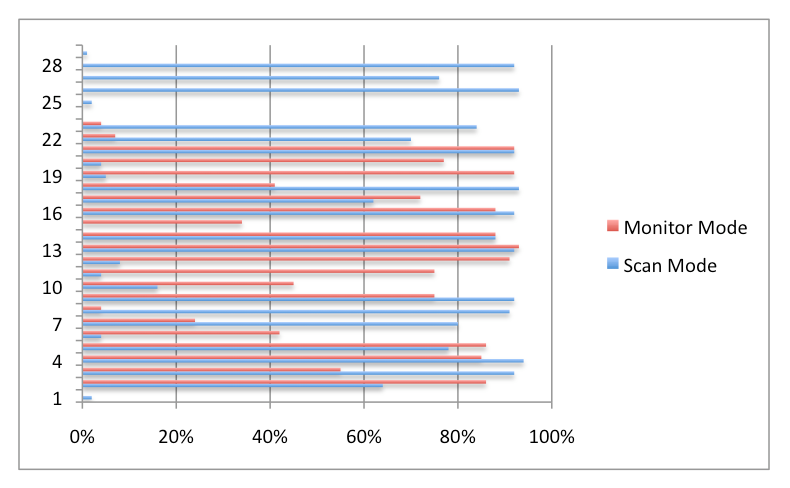
\includegraphics[scale=0.7]{cpu}}
\caption{The CPU usage comparison of Monitor and Scan mode}
\label{fig:cpu}
\end{figure}

The same as CPU usage, the memory usage data is also disappointed. As shown in Figure~\ref{fig:memory}, the memory usage in 
monitor mode is even higher than scan mode. We think this is due to our implementation use only \verb+ScanFileThread+ in 
scan mode while using an extra \verb+FileMonitorThread+ in monitor thread. 

\begin{figure}%[htp]
\centering
\subfigure[Memory Usage in Monitor Mode]{\label{fig:memory-monitor}
    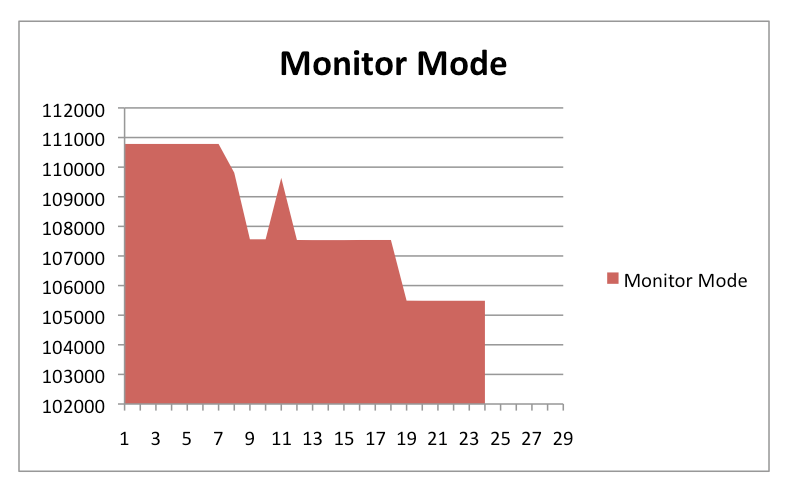
\includegraphics[scale=0.5]{memory_monitor}}
\hspace{0.20in}
\subfigure[Memory Usage in Scan Mode]{\label{fig:memory-scan}
	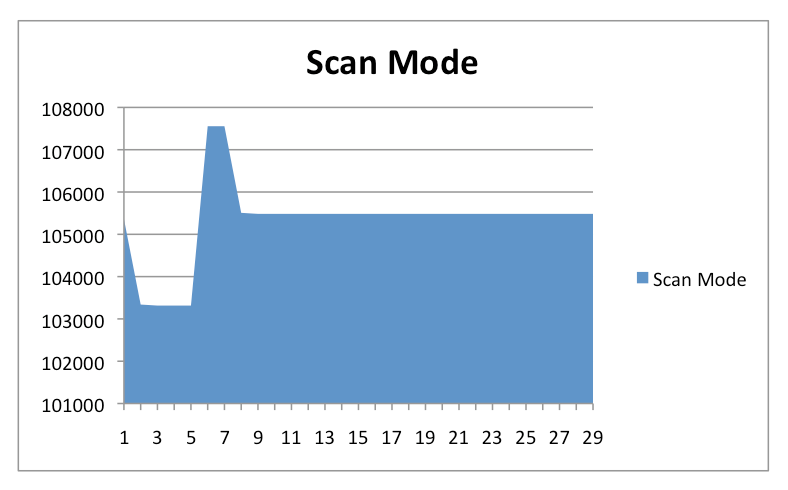
\includegraphics[scale=0.5]{memory_scan}}
\subfigure[Comparison of Memory Usage]{\label{fig:memory-comp}
    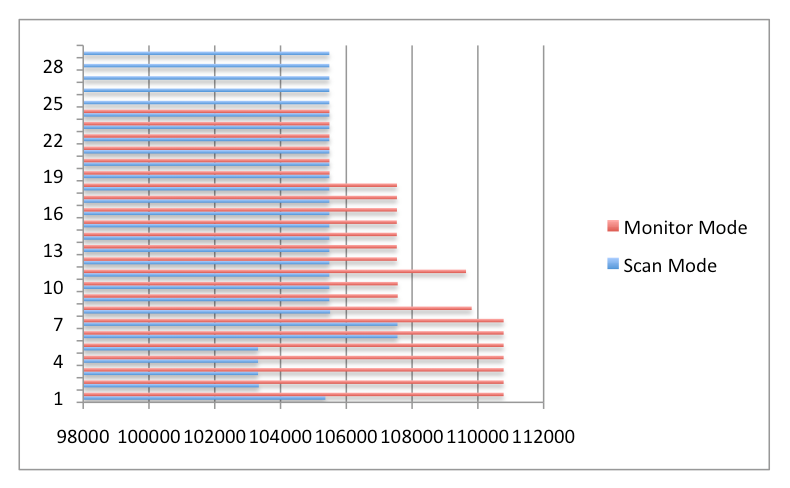
\includegraphics[scale=0.7]{memory}}
\caption{The Memory usage comparison of Monitor and Scan mode}
\label{fig:memory}
\end{figure}

In the test of synchronization speed, we finally got the data represent the the performance of monitor version is better. 
As we can see in Figure~\ref{fig:speed}, the speed of monitor mode is faster than scan mode on client side. However, the 
server didn't show significant differences. This may be due to our current server side script using a pull-sync instead of push-sync as client side. 
\begin{figure}[htp]
\centering
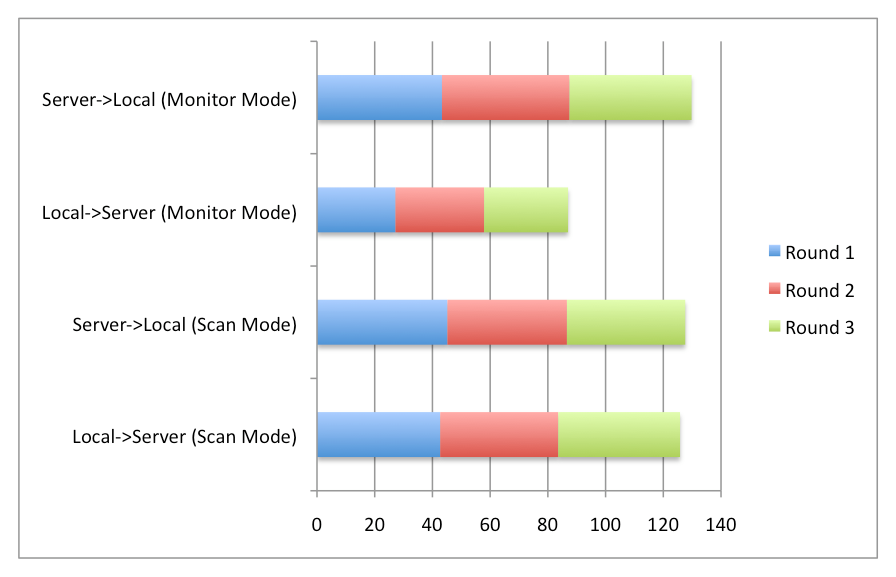
\includegraphics[scale=0.7]{speed}
\caption{Comparison of Synchronization Speed}\label{fig:speed}
\end{figure}
